\documentclass{article}\usepackage[]{graphicx}\usepackage[]{color}
%% maxwidth is the original width if it is less than linewidth
%% otherwise use linewidth (to make sure the graphics do not exceed the margin)
\makeatletter
\def\maxwidth{ %
  \ifdim\Gin@nat@width>\linewidth
    \linewidth
  \else
    \Gin@nat@width
  \fi
}
\makeatother

\definecolor{fgcolor}{rgb}{0.345, 0.345, 0.345}
\newcommand{\hlnum}[1]{\textcolor[rgb]{0.686,0.059,0.569}{#1}}%
\newcommand{\hlstr}[1]{\textcolor[rgb]{0.192,0.494,0.8}{#1}}%
\newcommand{\hlcom}[1]{\textcolor[rgb]{0.678,0.584,0.686}{\textit{#1}}}%
\newcommand{\hlopt}[1]{\textcolor[rgb]{0,0,0}{#1}}%
\newcommand{\hlstd}[1]{\textcolor[rgb]{0.345,0.345,0.345}{#1}}%
\newcommand{\hlkwa}[1]{\textcolor[rgb]{0.161,0.373,0.58}{\textbf{#1}}}%
\newcommand{\hlkwb}[1]{\textcolor[rgb]{0.69,0.353,0.396}{#1}}%
\newcommand{\hlkwc}[1]{\textcolor[rgb]{0.333,0.667,0.333}{#1}}%
\newcommand{\hlkwd}[1]{\textcolor[rgb]{0.737,0.353,0.396}{\textbf{#1}}}%
\let\hlipl\hlkwb

\usepackage{framed}
\makeatletter
\newenvironment{kframe}{%
 \def\at@end@of@kframe{}%
 \ifinner\ifhmode%
  \def\at@end@of@kframe{\end{minipage}}%
  \begin{minipage}{\columnwidth}%
 \fi\fi%
 \def\FrameCommand##1{\hskip\@totalleftmargin \hskip-\fboxsep
 \colorbox{shadecolor}{##1}\hskip-\fboxsep
     % There is no \\@totalrightmargin, so:
     \hskip-\linewidth \hskip-\@totalleftmargin \hskip\columnwidth}%
 \MakeFramed {\advance\hsize-\width
   \@totalleftmargin\z@ \linewidth\hsize
   \@setminipage}}%
 {\par\unskip\endMakeFramed%
 \at@end@of@kframe}
\makeatother

\definecolor{shadecolor}{rgb}{.97, .97, .97}
\definecolor{messagecolor}{rgb}{0, 0, 0}
\definecolor{warningcolor}{rgb}{1, 0, 1}
\definecolor{errorcolor}{rgb}{1, 0, 0}
\newenvironment{knitrout}{}{} % an empty environment to be redefined in TeX

\usepackage{alltt}
\usepackage{gensymb}
\usepackage[T1]{fontenc}
\usepackage{hyperref}

\title{Visual Presentation of Data using R}



\IfFileExists{upquote.sty}{\usepackage{upquote}}{}
\begin{document}
\maketitle

\section{The Perfect Graphic}

\subsection{Best Practices}

There is no such thing as the perfect graphic, but there are conventions that can be used to guide us to create accurtate, accessible, and visually pleasing grahics. But like many things, it takes some practices. 

Here are some general rules:

\begin{itemize}
  \item Be sure that you introduce the graphic/table with text -- i.e. text first, then graphic. 
  \item Cite the graphic/table with a figure or table number. 
  \item Describe the graphic/table with a caption.
  \item Manage data range and transformations to effectively analyze and display the data.
  \item Make sure the axes are labeled with appropriate units
  \item Manage axis labels, value font size, and orientation to make them easy to reads.
  \item Avoid graphic titles unless you have more than one panel, i.e. graphics that are side by side or on top of each other. 
  \item Do not connect data points with lines unless you can 'reasonable' interpolate between the points, e.g. a continous data set with some level of autocorrelation. 
  \item Are the graphics accessible?  For example, black and white can be better than color in terms of accessibility (universal design) and sustainability. 
  \item Use the caption to describe what the reader is supposed to see in the figure. 
\end{itemize}

\subsection{How to Cite Software}

In the text, students often make a bigger deal out the software than it deserses. Probably, because we feel like we climbed a big mountain to have some success and want demonstrate that. However, in general, environmental scientists downplay the software, unless they wrote a specific function or library. 

Thus, for our purposes, the following is usually sufficient...

\noindent ``Statistical analysis was conducted using using R (CRAN 2019)."

You don't need to mention how you imported it, used Rstudio, or talk about the functions. In the text, you might mention that you used a linear model, regression, analysis of variance (AOV), but the details of the R code is usually not mentioned.

However, you should also cite the program in your endnote: 

\smallskip
To cite R in publications use:

\medskip
\noindent R Core Team. 2017. R: A language and environment for statistical computing. R Foundation for Statistical Computing, Vienna, Austria. URL \url{https://www.R-project.org/}.

\smallskip

\noindent You can get an updated version of the citation using the following function in R: citation(). Although the format isn't quite the same.
  

\subsection{Reporting Results}

In statistics, we reject the null hypothesis -- and don't prove anything. So, we need to be careful how we report our results. 

First, when we report statistics, do not report the p-value if the result in non-significant. Just report that null hypothesis cannot be rejected. For example, "there was no relationship between y and x". If the p-value is less then 0.001, just report it as `p $<$ 0.001'. If the p-value is between 0.05 and 0.001, then I suggest you report the actual value (rounded to the nearest one-hundredth or thousandth as appropriate. For example, "evidence suggest that y depends on x (p = 0.03)." 

Second, when we report the r$^2$ value, round to the nearest one-hundredth and describe it as the 'amount of variation explained by the model'. In fact, if you multiply by 100, it's can thought of as a percent variation explained.

Finally, avoid making the statistics the subject of the sentence! Describe the results as the subject/verb and then add a parenthetical about the stats, e.g.

\noindent Water quality declined through the study period (p = 0.03; r$^2$ = 0.09), although little of the variation was explained by the model. 

\subsection{On Rounding and Decimaled Numbers}

When numbers are less than 1 and reported as decimals, always report the leading zero, e.g. 0.02 instead of .02. It reduces ambiguities and helps ensure you haven't misreported the values with a typo.

We always want to round to the highest signficant figure. Thus, if temperatures are reported to the nearest degree, then can't report and average of 4.00324432$\degree$ C. For an average, we can report one decimal to the right of the reported instrument precision, thus 4.0$\degree$ C would be appropriate. By reporting the following zero, we are explicit about the significant figures -- thus is a reporting requirement. 

\subsection{Special Symbols}

Science often relies on specialized characters, e.g. $\degree$ for degrees, $\alpha$ for our statistical test criteria. Table \ref{tab:symbols} shows the codes for symbols for Rmarkdown and \LaTeX.

\begin{table}
\caption{Special Symbols for Rmarkdown and \LaTeX}
\label{tab:symbols}
\begin{tabular}{lll}\hline
Symbol  & Markdown Code & \LaTeX code \\ \hline\hline
r$^2$     & r\^{}2\^{} &  r\$\^{}2\$ \\
CO$_2$    & CO<sub>2<\textbackslash sub> & CO\$\_2\$\\

$\alpha$ & \$\textbackslash alpha\$ & \$\textbackslash alpha\$ \\

$\mu$ & \$\textbackslash mu\$ & \$\textbackslash mu\$ \\


$\degree$ & \&deg; & \$\textbackslash degree\$ \\ 
\hline
\end{tabular}
\end{table}

\section{Exploring the Histogram}

Data exploration can include many steps, but starting with a histogram gives the researcher the ability to evaluate the distribution of the data.

Below is a default histogram for TMAX values, where we might be able to visually how normally distributed the data might be.

\begin{knitrout}
\definecolor{shadecolor}{rgb}{0.969, 0.969, 0.969}\color{fgcolor}\begin{kframe}
\begin{alltt}
\hlkwd{hist}\hlstd{(MonthlyTMAXMean}\hlopt{$}\hlstd{TMAX)}
\end{alltt}
\end{kframe}
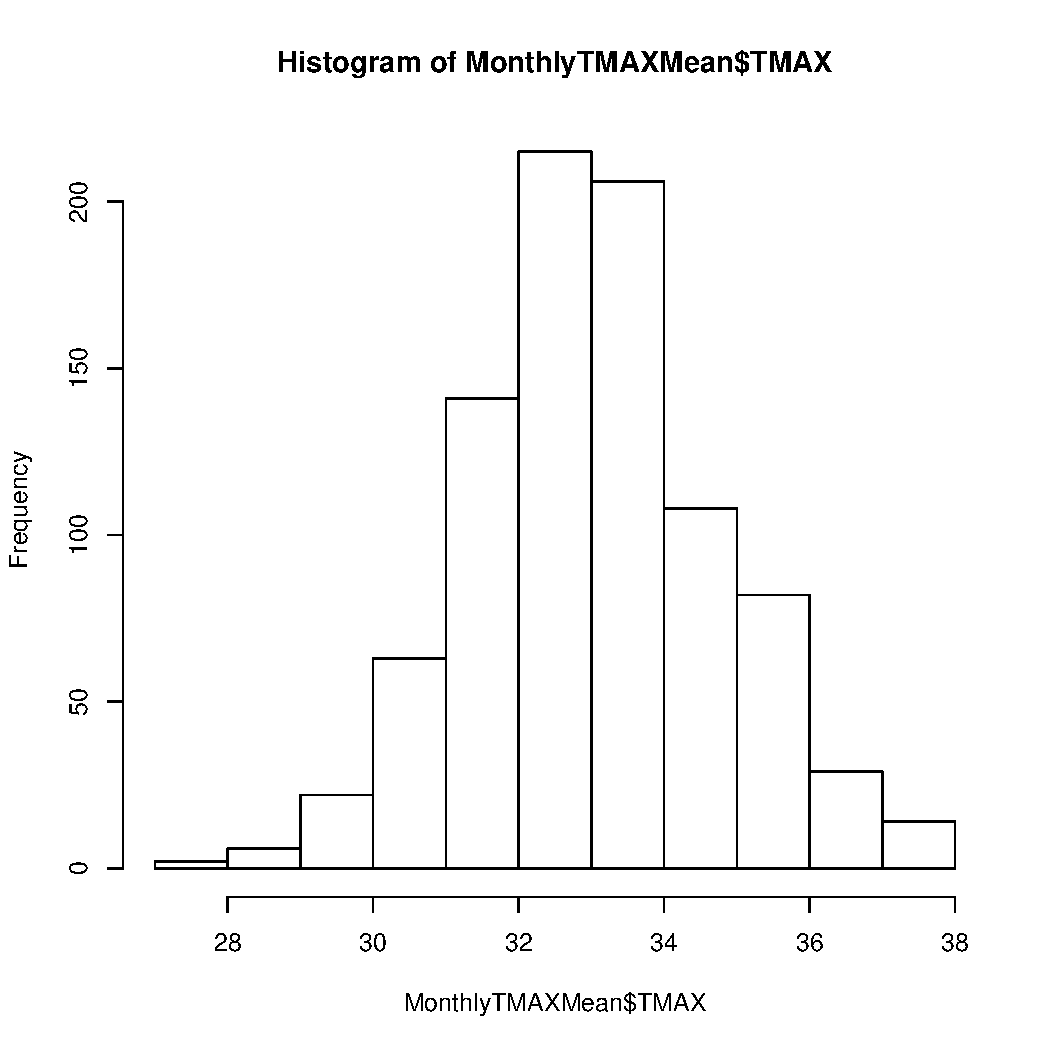
\includegraphics[width=\maxwidth]{figure/unnamed-chunk-2-1} 

\end{knitrout}

The default graphic is hideous -- so, let's start fixing it. 

\subsection{Title and Axis Labels}

For stand alone figures, we usually add titles, but in papers and lab reports it's a good practice to remove the title and use the caption to describe the graphic. Changes to the title can be made with arguments within the plot command, i.e. `main=NULL'.

In addition, we can change the x-axis label, with the 'xlab' argument. Specifying the units is also required. And in this case, we want to add the \degree symbol and create a text string with the axis label in quotes that can be referenced in the hist() funtion. Notice that I rotated the y-axis values (las=1). 

\begin{knitrout}
\definecolor{shadecolor}{rgb}{0.969, 0.969, 0.969}\color{fgcolor}\begin{kframe}
\begin{alltt}
\hlstd{TMAXlabel} \hlkwb{<-} \hlstr{"Maximum Temperature (°C)"}
\hlkwd{hist}\hlstd{(MonthlyTMAXMean}\hlopt{$}\hlstd{TMAX,} \hlkwc{main}\hlstd{=}\hlkwa{NULL}\hlstd{,} \hlkwc{xlab}\hlstd{=TMAXlabel,} \hlkwc{las}\hlstd{=}\hlnum{1}\hlstd{)}
\end{alltt}
\end{kframe}\begin{figure}
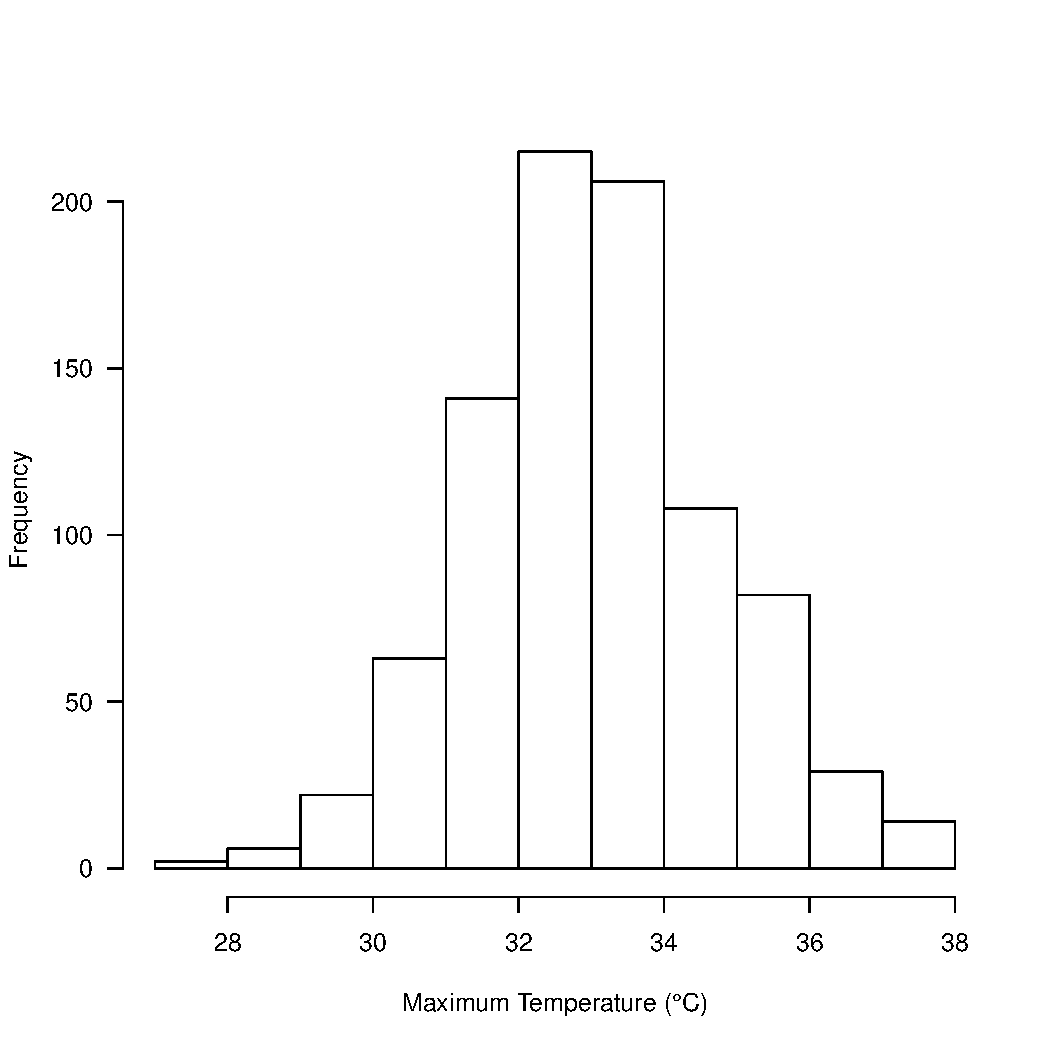
\includegraphics[width=\maxwidth]{figure/unnamed-chunk-3-1} \caption[Histogram of Maximum Temperatures (°C) (XXX, Thailand, 1940-2018)]{Histogram of Maximum Temperatures (°C) (XXX, Thailand, 1940-2018)}\label{fig:unnamed-chunk-3}
\end{figure}


\end{knitrout}
\clearpage

\subsection{Putting Multiple Figures in a Row}

To create two graphics in one row, we can change the graphic parameters with the par() function. In this case, we'll create two column panels in one row using the 'mfrow' option and a vector that defines the number of rows and the number of columns, e.g. 'par(mfrow=c(1, 2))'. It's often a good idea to set the graphic parameter back to the default afterwards. In this case, I added a title because we have a panel with two graphics. Often people will put letters, e.g. A and B to refer to each one separately, but I prefer to put the actually description in the title, so the reader doesn't have to go back and forth between the caption and the figures. 

Note: the title is too long! So, I will need to figure out how to adjust the size of the font at some point using 'cex' arguments. See the boxplots below to see how that can be done.

\begin{knitrout}
\definecolor{shadecolor}{rgb}{0.969, 0.969, 0.969}\color{fgcolor}\begin{kframe}
\begin{alltt}
\hlkwd{par}\hlstd{(}\hlkwc{mfrow}\hlstd{=}\hlkwd{c}\hlstd{(}\hlnum{1}\hlstd{,}\hlnum{2}\hlstd{))}
\hlkwd{hist}\hlstd{(MonthlyTMAXMean}\hlopt{$}\hlstd{TMAX,} \hlkwc{main}\hlstd{=}\hlstr{'Maximum Temperature'}\hlstd{,} \hlkwc{xlab}\hlstd{=TMAXlabel)}
\hlstd{TMINlabel} \hlkwb{<-} \hlstr{"Minimum Temperature (°C)"}
\hlkwd{hist}\hlstd{(MonthlyTMINMean}\hlopt{$}\hlstd{TMIN,} \hlkwc{main}\hlstd{=}\hlstr{'Minimum Temperature'}\hlstd{,} \hlkwc{xlab}\hlstd{=TMINlabel)}
\end{alltt}
\end{kframe}\begin{figure}
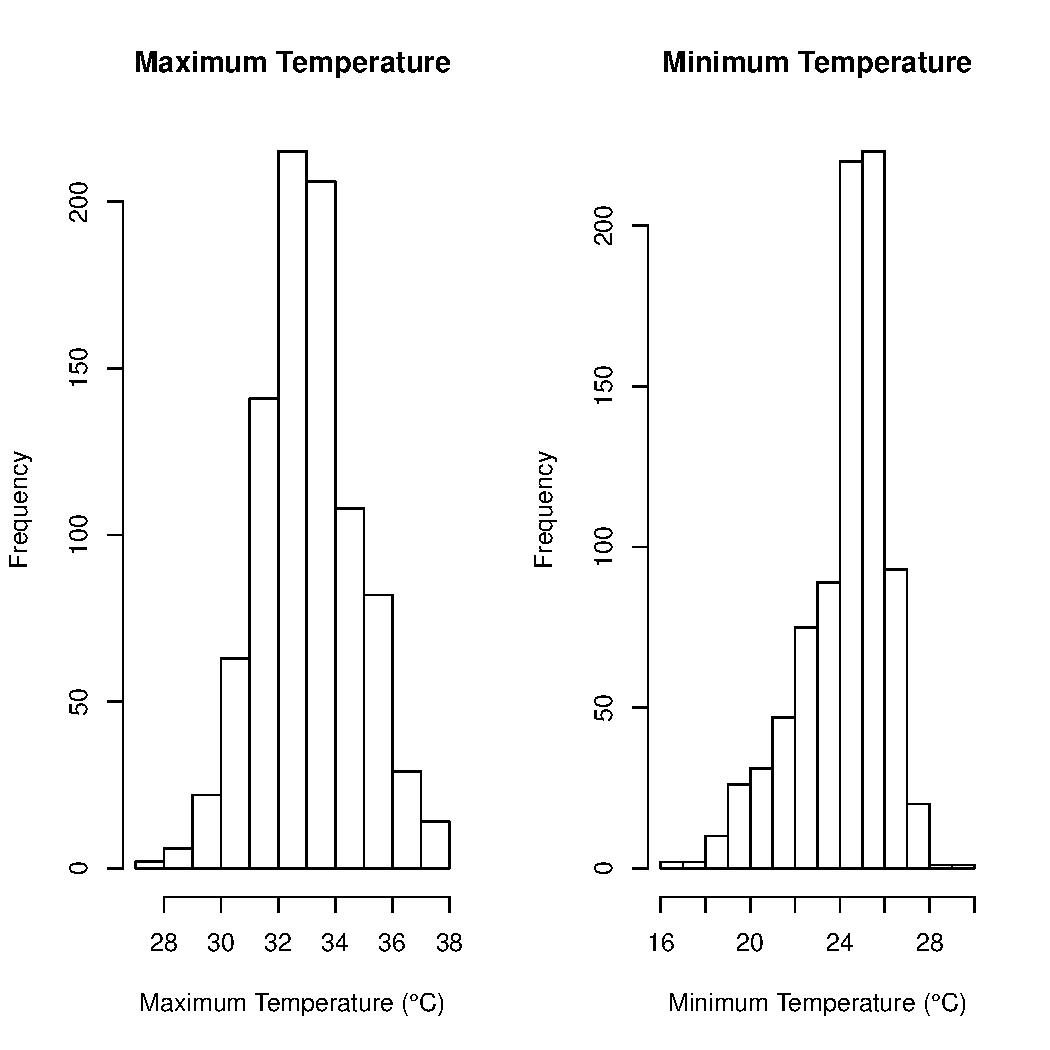
\includegraphics[width=\maxwidth]{figure/unnamed-chunk-4-1} \caption[Mean monthly maximum and minimum tempetures (C) ((Bangkok, Thailand, 1940-2018))]{Mean monthly maximum and minimum tempetures (C) ((Bangkok, Thailand, 1940-2018))}\label{fig:unnamed-chunk-4}
\end{figure}

\begin{kframe}\begin{alltt}
\hlkwd{par}\hlstd{(}\hlkwc{mfrow}\hlstd{=}\hlkwd{c}\hlstd{(}\hlnum{1}\hlstd{,}\hlnum{1}\hlstd{))}
\end{alltt}
\end{kframe}
\end{knitrout}
\newpage
Because the figure is rather distorted, I have constrained the size using a fig.height and fig.width option. 

\begin{knitrout}
\definecolor{shadecolor}{rgb}{0.969, 0.969, 0.969}\color{fgcolor}\begin{kframe}
\begin{alltt}
\hlkwd{par}\hlstd{(}\hlkwc{mfrow}\hlstd{=}\hlkwd{c}\hlstd{(}\hlnum{1}\hlstd{,}\hlnum{2}\hlstd{))}
\hlkwd{hist}\hlstd{(MonthlyTMAXMean}\hlopt{$}\hlstd{TMAX,} \hlkwc{main}\hlstd{=}\hlstr{'Monthly Maximum Temperature'}\hlstd{,} \hlkwc{xlab}\hlstd{=TMAXlabel)}
\hlstd{TMINlabel} \hlkwb{<-} \hlstr{"Minimum Temperature (°C)"}
\hlkwd{hist}\hlstd{(MonthlyTMINMean}\hlopt{$}\hlstd{TMIN,} \hlkwc{main}\hlstd{=}\hlstr{'Monthly Minimum Temperature'}\hlstd{,} \hlkwc{xlab}\hlstd{=TMINlabel)}
\end{alltt}
\end{kframe}\begin{figure}
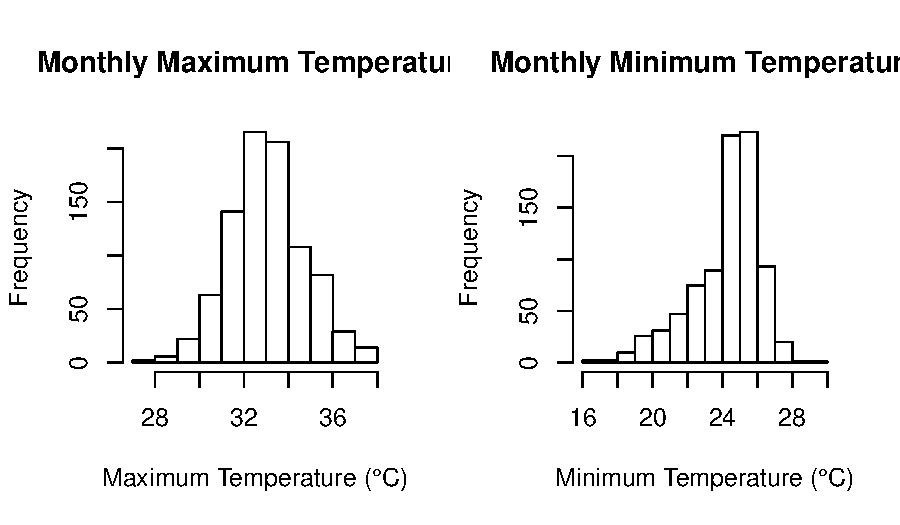
\includegraphics[width=\maxwidth]{figure/unnamed-chunk-5-1} \caption[Mean monthly maximum and minimum tempetures (C) ((XXX, Thailand, 1940-2018))]{Mean monthly maximum and minimum tempetures (C) ((XXX, Thailand, 1940-2018)).}\label{fig:unnamed-chunk-5}
\end{figure}

\begin{kframe}\begin{alltt}
\hlkwd{par}\hlstd{(}\hlkwc{mfrow}\hlstd{=}\hlkwd{c}\hlstd{(}\hlnum{1}\hlstd{,}\hlnum{1}\hlstd{))}
\end{alltt}
\end{kframe}
\end{knitrout}

Note that the title is too big and is cut off. In general, most publications prefer you put the description in the caption and avoid long titles. So, for the next example, I'll create a caption to refer to both figures as panel letters and get rid of the figure titles (main=NULL).

Altnernatively, I could change the relative size of the titles, using 'cex.main = 0.8', which multiplies the size by 0.8. 

To create the panel letters, we'll use mtext for margin text. 

\begin{knitrout}
\definecolor{shadecolor}{rgb}{0.969, 0.969, 0.969}\color{fgcolor}\begin{kframe}
\begin{alltt}
\hlkwd{par}\hlstd{(}\hlkwc{mfrow}\hlstd{=}\hlkwd{c}\hlstd{(}\hlnum{1}\hlstd{,}\hlnum{2}\hlstd{))}
\hlkwd{hist}\hlstd{(MonthlyTMAXMean}\hlopt{$}\hlstd{TMAX,} \hlkwc{main}\hlstd{=}\hlkwa{NULL}\hlstd{,} \hlkwc{xlab}\hlstd{=TMAXlabel)}
\hlstd{TMINlabel} \hlkwb{<-} \hlstr{"Minimum Temperature (°C)"}
\hlkwd{mtext}\hlstd{(}\hlstr{"A"}\hlstd{,} \hlkwc{side}\hlstd{=}\hlnum{3}\hlstd{,} \hlkwc{line}\hlstd{=}\hlnum{0}\hlstd{,} \hlkwc{adj}\hlstd{=}\hlnum{0}\hlstd{,} \hlkwc{cex}\hlstd{=}\hlnum{1.4}\hlstd{)}
\hlkwd{hist}\hlstd{(MonthlyTMINMean}\hlopt{$}\hlstd{TMIN,} \hlkwc{main}\hlstd{=}\hlkwa{NULL}\hlstd{,} \hlkwc{xlab}\hlstd{=TMINlabel)}
\hlkwd{mtext}\hlstd{(}\hlstr{"B"}\hlstd{,} \hlkwc{side}\hlstd{=}\hlnum{3}\hlstd{,} \hlkwc{line}\hlstd{=}\hlnum{0}\hlstd{,} \hlkwc{adj}\hlstd{=}\hlnum{0}\hlstd{,} \hlkwc{cex}\hlstd{=}\hlnum{1.4}\hlstd{)}
\end{alltt}
\end{kframe}\begin{figure}
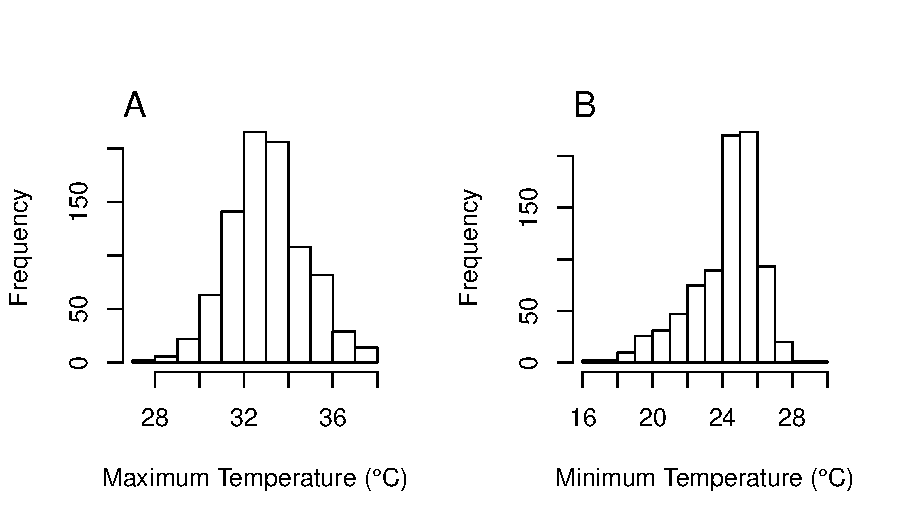
\includegraphics[width=\maxwidth]{figure/unnamed-chunk-6-1} \caption[Mean monthly maximum (Panel A) and minimum (Panel B) tempetures (C) ((Bangkok, Thailand, 1940-2018))]{Mean monthly maximum (Panel A) and minimum (Panel B) tempetures (C) ((Bangkok, Thailand, 1940-2018)).}\label{fig:unnamed-chunk-6}
\end{figure}

\begin{kframe}\begin{alltt}
\hlkwd{par}\hlstd{(}\hlkwc{mfrow}\hlstd{=}\hlkwd{c}\hlstd{(}\hlnum{1}\hlstd{,}\hlnum{1}\hlstd{))}
\end{alltt}
\end{kframe}
\end{knitrout}

\section{Boxplot}

Box plots are great ways to display quantitative data from controlled experiments. For example, if you had high and low treatment categories and measured some response. Let's use the following example, ants colonies collected from three locations farm, grassland, and forest. 

\begin{knitrout}
\definecolor{shadecolor}{rgb}{0.969, 0.969, 0.969}\color{fgcolor}\begin{figure}
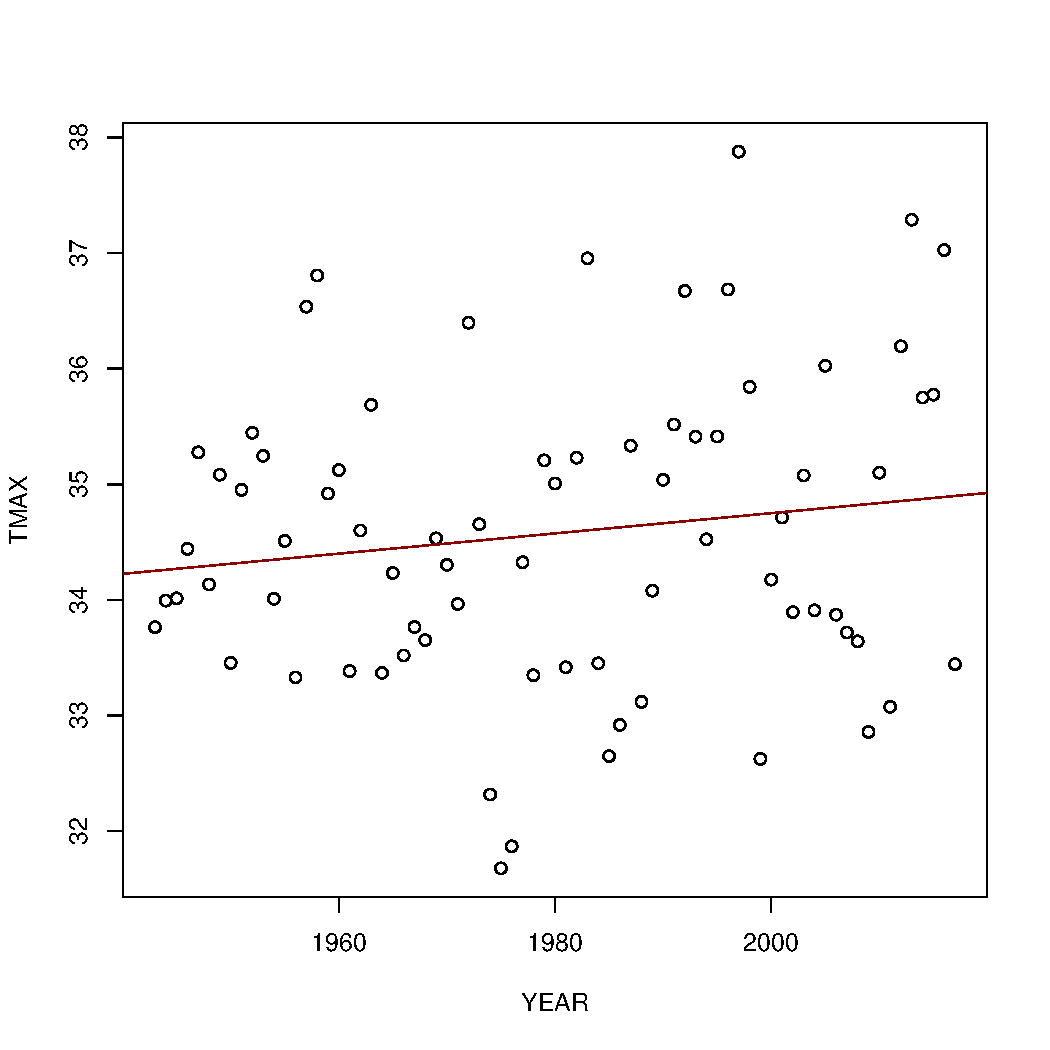
\includegraphics[width=\maxwidth]{figure/unnamed-chunk-7-1} \caption[Number of ant colonies by habitat type]{Number of ant colonies by habitat type.}\label{fig:unnamed-chunk-7}
\end{figure}


\end{knitrout}


The boxplot can be improved dramatically by rotating the y-axis values ('las=1'), increasing the size of the axis labels ('cex.lab') and axis values ('cex.axis') (Figure~\ref{fig:boxplot}.
\begin{knitrout}
\definecolor{shadecolor}{rgb}{0.969, 0.969, 0.969}\color{fgcolor}\begin{kframe}
\begin{alltt}
\hlkwd{boxplot}\hlstd{(Colonies} \hlopt{~} \hlstd{Location,} \hlkwc{data}\hlstd{=ants,} \hlkwc{las}\hlstd{=}\hlnum{1}\hlstd{,}
        \hlkwc{ylab}\hlstd{=}\hlstr{"No. of Colonies"}\hlstd{,} \hlkwc{xlab}\hlstd{=}\hlstr{"Habitat"}\hlstd{,} \hlkwc{cex.lab}\hlstd{=}\hlnum{1.6}\hlstd{,}
        \hlkwc{cex.axis}\hlstd{=}\hlnum{1.4}\hlstd{,} \hlkwc{col}\hlstd{=}\hlstr{"gray"}\hlstd{)}
\end{alltt}
\end{kframe}\begin{figure}
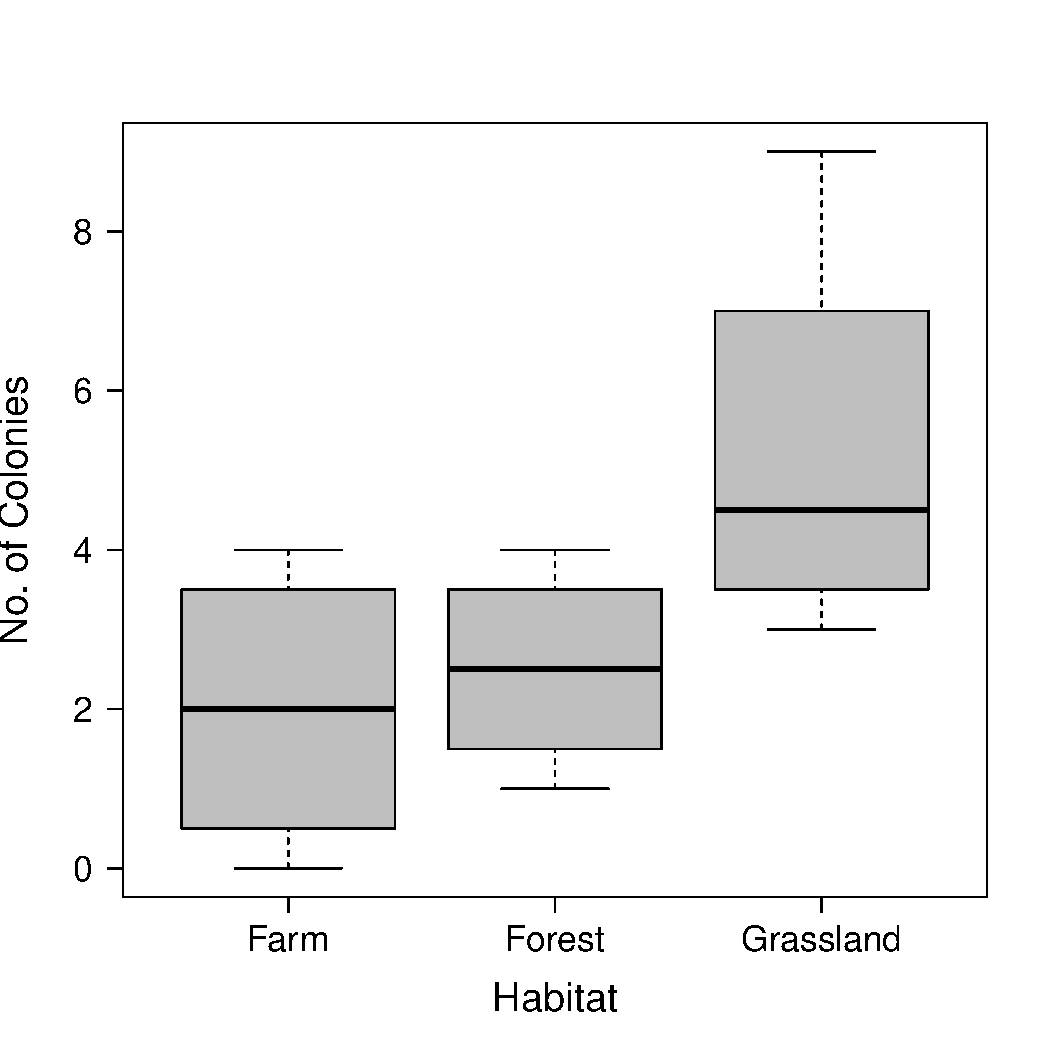
\includegraphics[width=\maxwidth]{figure/boxplot-1} \caption[Number of ant colonies by habitat type]{Number of ant colonies by habitat type.}\label{fig:boxplot}
\end{figure}


\end{knitrout}




\newpage
\section{Scatter Plot -- Non-time series}

%For scatter plots, which are more common, we use the same principles:


\subsection{Scatter Plot -- Time Series}

Time series data sets often require special treatment. For example, data are often autocorrelated, thus data can be represented by lines instead of points. However, this requires some careful thought. 

When we are graphing temperature data from one year to the next, we are averaging many days and connecting one year to the next might be appropriate if the data series is long enough, e.g. more than 50 years. However, with shorter time-series, i.e. 15 or less, connect the years with a line might be problematic.

\begin{knitrout}
\definecolor{shadecolor}{rgb}{0.969, 0.969, 0.969}\color{fgcolor}\begin{kframe}
\begin{alltt}
\hlkwd{plot}\hlstd{(TMAX} \hlopt{~} \hlstd{YEAR,} \hlkwc{data}\hlstd{=MonthlyTMAXMean[MonthlyTMAXMean}\hlopt{$}\hlstd{MONTH}\hlopt{==}\hlnum{5}\hlstd{,])}
\hlkwd{abline}\hlstd{(}\hlkwd{coef}\hlstd{(}\hlkwd{lm}\hlstd{(TMAX} \hlopt{~} \hlstd{YEAR,} \hlkwc{data}\hlstd{=MonthlyTMAXMean[MonthlyTMAXMean}\hlopt{$}\hlstd{MONTH}\hlopt{==}\hlnum{5}\hlstd{,])),}
    \hlkwc{col}\hlstd{=}\hlstr{'darkred'}\hlstd{)}
\end{alltt}
\end{kframe}
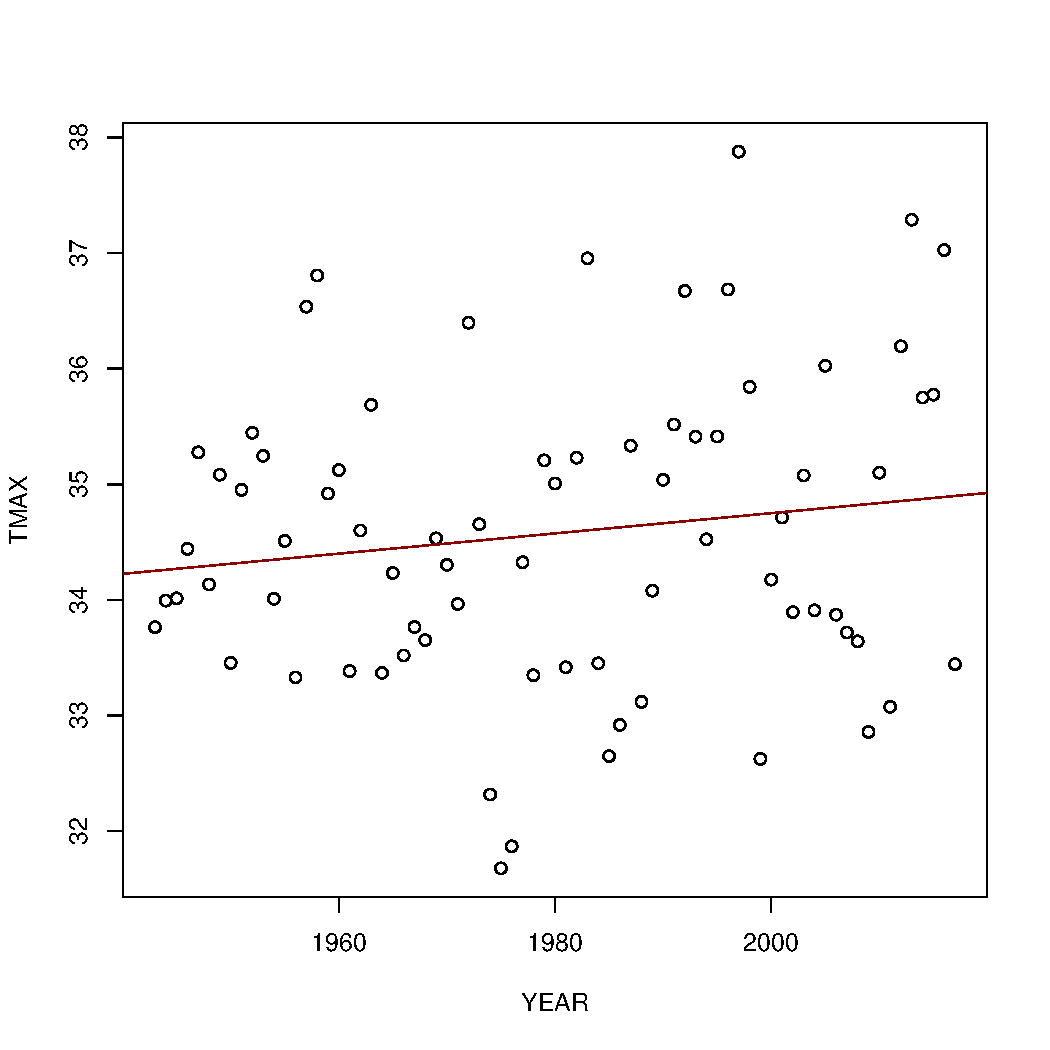
\includegraphics[width=\maxwidth]{figure/plot1-1} 

\end{knitrout}

Let's fix the y-axis label as we did above (TMAX is not a very helpful label!). Furthermore, the x-axis needs to be calmed down some, so let's change the case for these. We will also change the symbols to make it less busy with the `pch' argument. You can look online to see the choices one has in R. 

I am also not impress with the vertical orientation of the y-axis, so it's important to change these as well. 

Finally, it's important that the image works in black and white. So, let's see if we can modify the graphic to make it less resource intensive. Finally, let's add a caption and reference to the figure (Figure \ref{fig:maxtemp}).

\begin{figure}[h]
\begin{knitrout}
\definecolor{shadecolor}{rgb}{0.969, 0.969, 0.969}\color{fgcolor}\begin{kframe}
\begin{alltt}
\hlstd{ylabel} \hlkwb{<-} \hlstr{"Maximum Temperature (°C)"}
\hlkwd{plot}\hlstd{(TMAX} \hlopt{~} \hlstd{YEAR,} \hlkwc{data}\hlstd{=MonthlyTMAXMean[MonthlyTMAXMean}\hlopt{$}\hlstd{MONTH}\hlopt{==}\hlnum{5}\hlstd{,],}
     \hlkwc{ylab}\hlstd{=ylabel,} \hlkwc{xlab}\hlstd{=}\hlstr{'Year'}\hlstd{,} \hlkwc{pch}\hlstd{=}\hlnum{20}\hlstd{,} \hlkwc{las}\hlstd{=}\hlnum{1}\hlstd{,} \hlkwc{col}\hlstd{=}\hlstr{'gray'}\hlstd{)}

\hlkwd{abline}\hlstd{(}\hlkwd{coef}\hlstd{(}\hlkwd{lm}\hlstd{(TMAX} \hlopt{~} \hlstd{YEAR,}
    \hlkwc{data}\hlstd{=MonthlyTMAXMean[MonthlyTMAXMean}\hlopt{$}\hlstd{MONTH}\hlopt{==}\hlnum{5}\hlstd{,])),} \hlkwc{col}\hlstd{=}\hlstr{'black'}\hlstd{)}
\end{alltt}
\end{kframe}
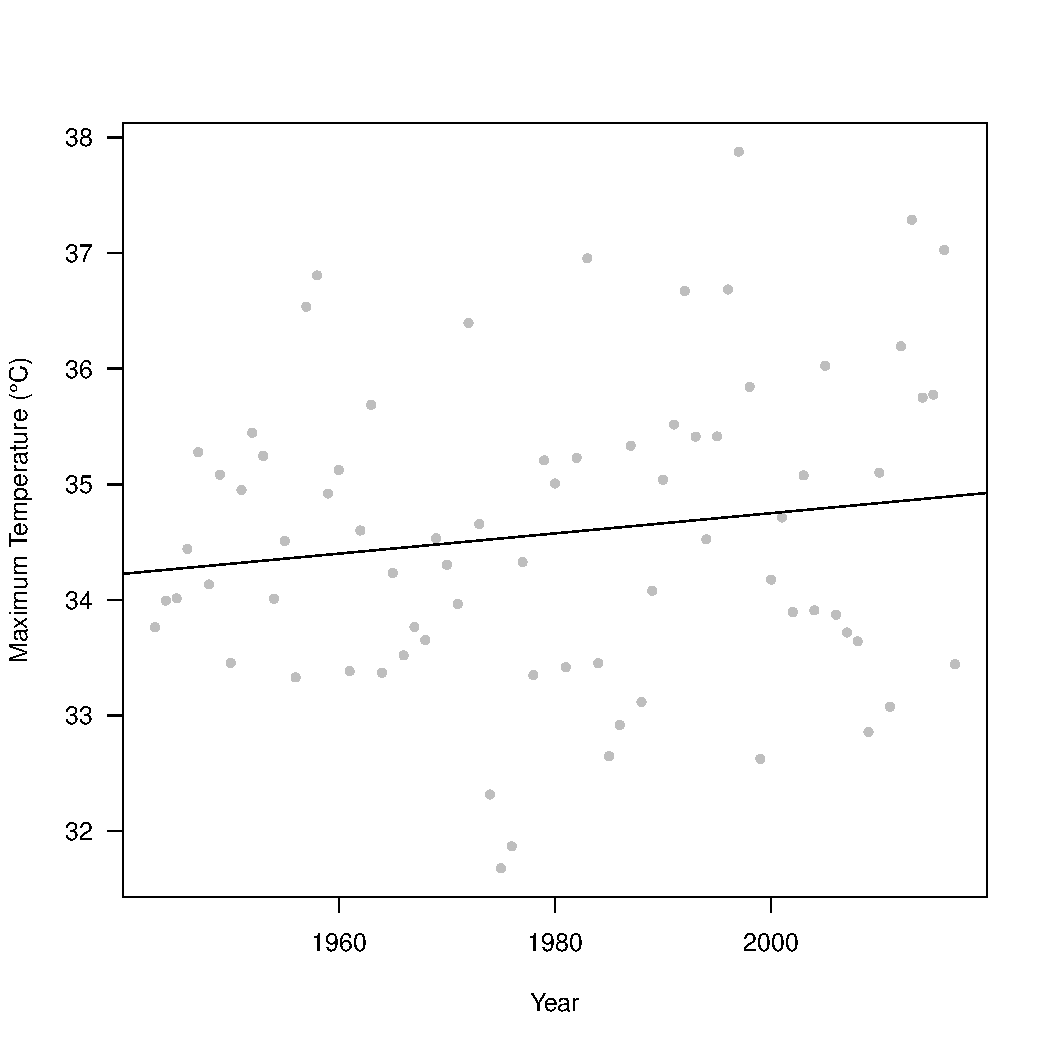
\includegraphics[width=\maxwidth]{figure/plot2-1} 

\end{knitrout}
\caption{Monthly Average of Daily Maximum Temperatures (\degree C).  Notice the slightly darker line in the x-axis for the middle section. I am not sure how to get rid of this, but it bugs me!}
\label{fig:maxtemp}
\end{figure}

\clearpage
Now, what if we only want to display part of the data. We can limit the x-axis range using the 'xlim' argument, where we create a vector of for the start and end of the range.  Finally, we can improve the plot by adding 'las=1' to rotate the y-axis labels. 

%\begin{figure}[h]
\begin{knitrout}
\definecolor{shadecolor}{rgb}{0.969, 0.969, 0.969}\color{fgcolor}\begin{kframe}
\begin{alltt}
\hlstd{ylabel} \hlkwb{<-} \hlstr{"Maximum Temperature (°C)"}
\hlkwd{plot}\hlstd{(TMAX} \hlopt{~} \hlstd{YEAR,} \hlkwc{data}\hlstd{=MonthlyTMAXMean[MonthlyTMAXMean}\hlopt{$}\hlstd{MONTH}\hlopt{==}\hlnum{5}\hlstd{,],}
     \hlkwc{xlim}\hlstd{=}\hlkwd{c}\hlstd{(}\hlnum{1940}\hlstd{,} \hlnum{2000}\hlstd{),}
     \hlkwc{ylab}\hlstd{=ylabel,} \hlkwc{xlab}\hlstd{=}\hlstr{'Year'}\hlstd{,} \hlkwc{pch}\hlstd{=}\hlnum{20}\hlstd{,} \hlkwc{las}\hlstd{=}\hlnum{1}\hlstd{,} \hlkwc{col}\hlstd{=}\hlstr{'gray'}\hlstd{)}

\hlkwd{abline}\hlstd{(}\hlkwd{coef}\hlstd{(}\hlkwd{lm}\hlstd{(TMAX} \hlopt{~} \hlstd{YEAR,}
    \hlkwc{data}\hlstd{=MonthlyTMAXMean[MonthlyTMAXMean}\hlopt{$}\hlstd{MONTH}\hlopt{==}\hlnum{5}\hlstd{,])),} \hlkwc{col}\hlstd{=}\hlstr{'black'}\hlstd{)}
\end{alltt}
\end{kframe}\begin{figure}
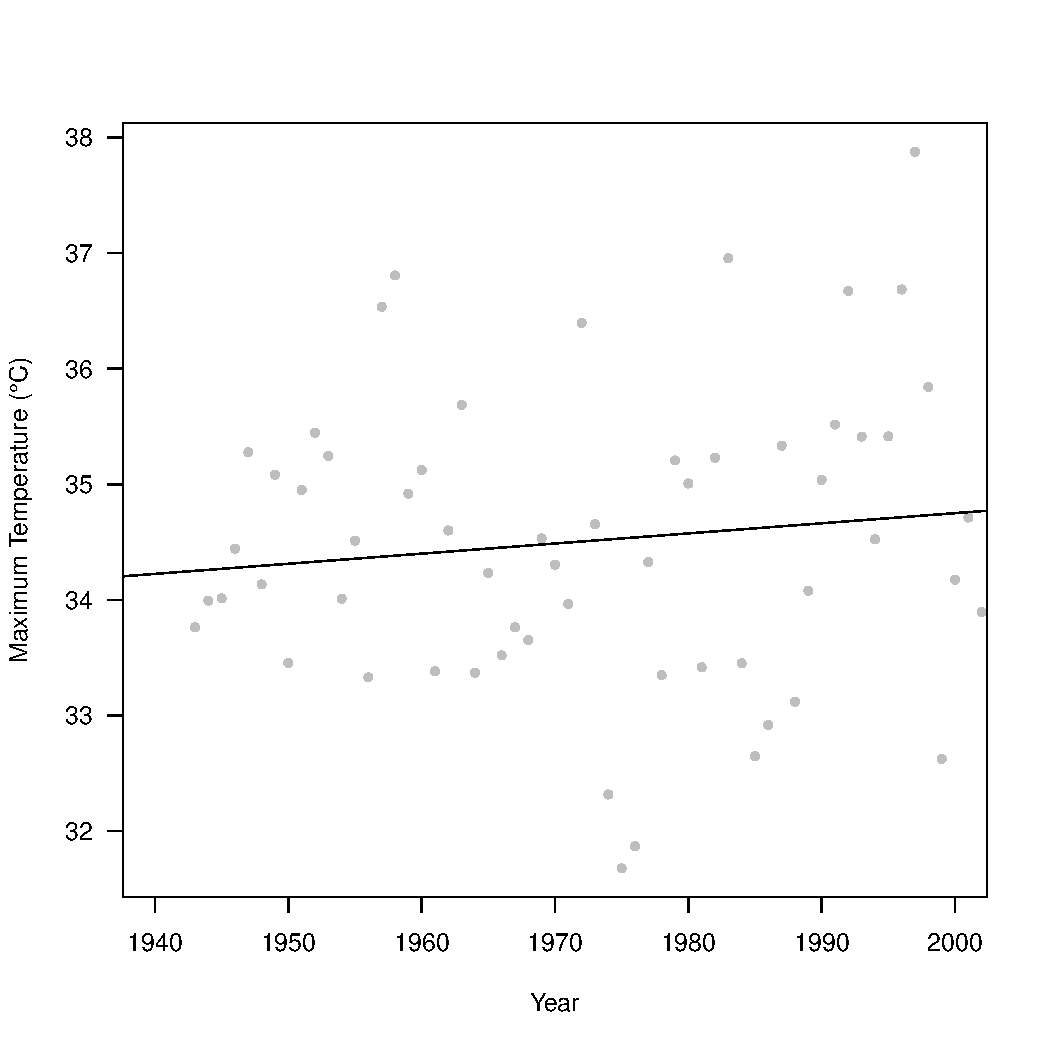
\includegraphics[width=\maxwidth]{figure/plot3-1} \caption[Monthly Average of Daily Maximum Temperatures (C)]{Monthly Average of Daily Maximum Temperatures (C).}\label{fig:plot3}
\end{figure}


\end{knitrout}
%\caption{Monthly Average of Daily Maximum Temperatures (\degree C).}
%\label{fig:maxtemp}
%\end{figure}

Alternatively, you may want to creat a best fit line that only covers the range for the existing data without extrapolating, which is usually a very good idea for most scientific endeavors!

For example, we have seen several papers that select parts of the record to make dubious claims. 

%\begin{figure}[ht]
\begin{knitrout}
\definecolor{shadecolor}{rgb}{0.969, 0.969, 0.969}\color{fgcolor}\begin{kframe}
\begin{alltt}
\hlstd{ylabel} \hlkwb{<-} \hlstr{"Maximum Temperature (°C)"}
\hlkwd{plot}\hlstd{(TMAX} \hlopt{~} \hlstd{YEAR,} \hlkwc{data}\hlstd{=MonthlyTMAXMean[MonthlyTMAXMean}\hlopt{$}\hlstd{MONTH}\hlopt{==}\hlnum{5}\hlstd{,],}
     \hlcom{#xlim=c(1940, 2000),}
     \hlkwc{ylab}\hlstd{=ylabel,} \hlkwc{xlab}\hlstd{=}\hlstr{'Year'}\hlstd{,} \hlkwc{pch}\hlstd{=}\hlnum{20}\hlstd{,} \hlkwc{las}\hlstd{=}\hlnum{1}\hlstd{,} \hlkwc{col}\hlstd{=}\hlstr{'gray'}\hlstd{)}

\hlstd{MonthlyTMAX.lm} \hlkwb{=} \hlstd{(}\hlkwd{lm}\hlstd{(TMAX} \hlopt{~} \hlstd{YEAR,}
    \hlkwc{data}\hlstd{=MonthlyTMAXMean[MonthlyTMAXMean}\hlopt{$}\hlstd{MONTH}\hlopt{==}\hlnum{5}\hlstd{, ]))}
\hlstd{interpolated} \hlkwb{=} \hlkwd{predict}\hlstd{(MonthlyTMAX.lm,}
      \hlstd{MonthlyTMAXMean[MonthlyTMAXMean}\hlopt{$}\hlstd{MONTH}\hlopt{==}\hlnum{5}\hlstd{,])}

\hlkwd{lines}\hlstd{(MonthlyTMAXMean}\hlopt{$}\hlstd{YEAR[MonthlyTMAXMean}\hlopt{$}\hlstd{MONTH}\hlopt{==}\hlnum{5}\hlstd{],}
      \hlstd{interpolated,} \hlkwc{col}\hlstd{=}\hlstr{'blue'}\hlstd{)}

\hlstd{MonthlyTMAX.lm2} \hlkwb{=} \hlstd{(}\hlkwd{lm}\hlstd{(TMAX} \hlopt{~} \hlstd{YEAR,}
    \hlkwc{data}\hlstd{=MonthlyTMAXMean[MonthlyTMAXMean}\hlopt{$}\hlstd{MONTH}\hlopt{==}\hlnum{5} \hlopt{&}
            \hlstd{MonthlyTMAXMean}\hlopt{$}\hlstd{YEAR}\hlopt{>}\hlnum{2000}\hlstd{, ]))}

\hlstd{interpolated2} \hlkwb{=} \hlkwd{predict}\hlstd{(MonthlyTMAX.lm2,}
            \hlstd{MonthlyTMAXMean[MonthlyTMAXMean}\hlopt{$}\hlstd{MONTH}\hlopt{==}\hlnum{5} \hlopt{&}
            \hlstd{MonthlyTMAXMean}\hlopt{$}\hlstd{YEAR}\hlopt{>}\hlnum{2000}\hlstd{,])}

\hlkwd{lines}\hlstd{(MonthlyTMAXMean}\hlopt{$}\hlstd{YEAR[MonthlyTMAXMean}\hlopt{$}\hlstd{MONTH}\hlopt{==}\hlnum{5} \hlopt{&}
            \hlstd{MonthlyTMAXMean}\hlopt{$}\hlstd{YEAR}\hlopt{>}\hlnum{2000}\hlstd{], interpolated2,} \hlkwc{col}\hlstd{=}\hlstr{'red'}\hlstd{)}

\hlkwd{legend}\hlstd{(}\hlnum{1948}\hlstd{,} \hlnum{38}\hlstd{,} \hlkwc{legend}\hlstd{=}\hlkwd{c}\hlstd{(}\hlstr{"1952-2018 Record"}\hlstd{,} \hlstr{"2000-2018 Record"}\hlstd{),}
       \hlkwc{lty}\hlstd{=}\hlnum{1}\hlstd{,} \hlkwc{col}\hlstd{=}\hlkwd{c}\hlstd{(}\hlstr{"blue"}\hlstd{,} \hlstr{"red"}\hlstd{))}
\end{alltt}
\end{kframe}
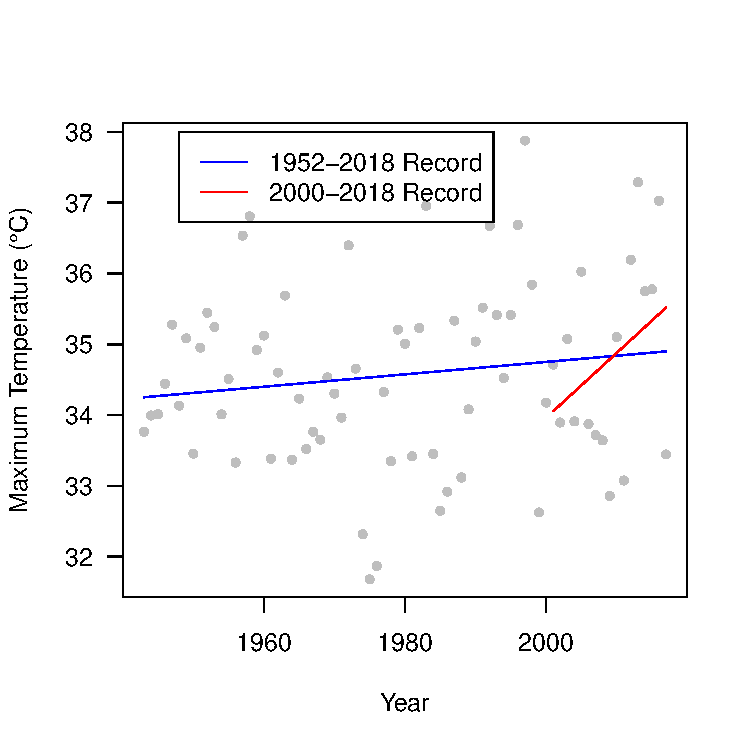
\includegraphics[width=\maxwidth]{figure/plot4-1} 

\end{knitrout}
%\caption{Monthly Average of Daily Maximum Temperatures (\degree C).}
%\label{fig:maxtemp}
%\end{figure}


\clearpage
\section{Bar Graphs}

\subsection{What are Barcharts}

Bar charts are used when you are graphing categorical data with continuous data that are a sum of something, for example dollars spent, no of events, and such. Rainfall is a good variable to put into barcharts with monthly or annual sums. 

\subsection{Introducing a Figure and Table}

We introduce our figures and tables in the text before the appear in the text. Just like a good friend, we introduce them to new people so they don't have to try to initiate a conversation without any context. Thus, we provide a bit of context to help the reader with the figure. 

One important note here -- when you report the results of a figure or a table, do not use the table or figure as the subject of the sentence. Instead use the results as the subject and reference the table or figure as a parenthetical. 

For example, 'The number of wildfires has dramatically increased after 2014 (Figure \ref{fig:barchart}). 

In my example, the figure should land after the text if possible. 

This is preferable to 'Figure \ref{fig:barchart}' shows that the number of wildfires has increased after 2014.' The emphasis is placed on the figure, which detracts to what the focus of the text should be on. Now there may be times when we want to put the focus on a table or complex figure, but usually we reserve that type of text for the figure caption. 

\begin{knitrout}
\definecolor{shadecolor}{rgb}{0.969, 0.969, 0.969}\color{fgcolor}\begin{kframe}
\begin{alltt}
\hlstd{fires} \hlkwb{=} \hlkwd{data.frame}\hlstd{(}\hlkwc{Year} \hlstd{=} \hlnum{2010}\hlopt{:}\hlnum{2018}\hlstd{,}
                   \hlkwc{Fires} \hlstd{=} \hlkwd{c}\hlstd{(}\hlnum{1}\hlstd{,} \hlnum{0}\hlstd{,} \hlnum{2}\hlstd{,} \hlnum{0}\hlstd{,} \hlnum{1}\hlstd{,} \hlnum{13}\hlstd{,} \hlnum{0}\hlstd{,} \hlnum{16}\hlstd{,} \hlnum{13}\hlstd{))}
\hlcom{# Note: barplot uses names.arg to assign the category names}
\hlkwd{barplot}\hlstd{(fires}\hlopt{$}\hlstd{Fires,} \hlkwc{names.arg} \hlstd{= fires}\hlopt{$}\hlstd{Year,} \hlkwc{las}\hlstd{=}\hlnum{1}\hlstd{,} \hlkwc{ylab}\hlstd{=}\hlstr{"No. of Fires"}\hlstd{)}
\end{alltt}
\end{kframe}\begin{figure}
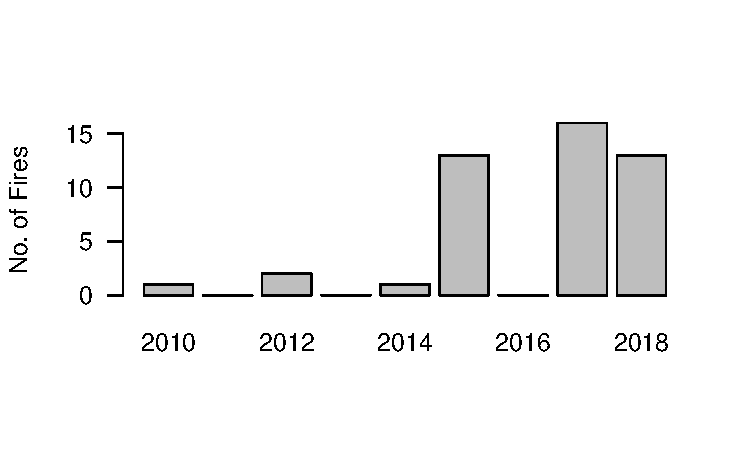
\includegraphics[width=\maxwidth]{figure/barchart-1} \caption[Number of Unsafe Air Quality Days in Washington State due to Fires]{Number of Unsafe Air Quality Days in Washington State due to Fires.}\label{fig:barchart}
\end{figure}


\end{knitrout}

\subsection{When to use Barcharts}

Rainfall data and other types of 'count' data are often best displayed as barcharts. 

Notice how Figure \ref{fig:barchart} cuts out every-other year. You'll need to decide if the reader will be bothered by that. If so, you can reduce the x-axis labels fonts or increase the width of the chart. 
\clearpage
\section{Tables}

Sometimes (often times?), tables are better than graphs. In the case below, I summarized the grades for each set of drafts using a table (Table 1) and through a series of histograms (Figure \ref{fig:scoreshist}). 




\begin{kframe}
\begin{alltt}
\hlkwd{print}\hlstd{(}\hlkwd{xtable}\hlstd{(grades.df,}
      \hlkwc{caption}\hlstd{=}\hlstr{'Table of Blog Draft Scores'}\hlstd{),} \hlkwc{type}\hlstd{=}\hlstr{'latex'}\hlstd{,}
      \hlkwc{caption.placement} \hlstd{=} \hlstr{"top"}\hlstd{,}
      \hlkwc{label}\hlstd{=}\hlstr{"tab:scores"}\hlstd{)}
\end{alltt}
\end{kframe}% latex table generated in R 3.4.1 by xtable 1.8-2 package
% 
\begin{tabular}{rlrrrrrr}
  \hline
 & Range & 1st Draft & 2nd Draft & 3nd Draft & 4th Draft & 5th Draft & Final \\ 
  \hline
1 & [0,10) &   4 &   0 &   0 &   0 &   0 &   0 \\ 
  2 & [10,20) &   0 &   3 &   0 &   0 &   0 &   1 \\ 
  3 & [20,30) &   7 &   2 &   1 &   0 &   0 &   3 \\ 
  4 & [30,40) &   4 &   6 &   2 &   0 &   0 &   5 \\ 
  5 & [40,50) &   0 &   1 &   5 &   2 &   1 &   6 \\ 
   \hline
\end{tabular}


\bigskip

The histogram is simple (Figure \ref{fig:scoreshist}), but for these data, I am not sure it's all that useful. Which do you think is more effective? 

The use of color in for this figure is really unnecessary. But it's worth illustrating. It's important that the use of color doesn't distract or confuse readers, especially those that are visually impaired, e.g. color blind.

\bigskip

You have 5 opportunities to re-submit to improve your grade, but only two weeks to accomplish this. Since it takes two days to read them, you'll need to submit every 2 days if you want to take full advange of this opportunity. 


\bigskip
\begin{knitrout}
\definecolor{shadecolor}{rgb}{0.969, 0.969, 0.969}\color{fgcolor}\begin{kframe}
\begin{alltt}
\hlkwd{par}\hlstd{(}\hlkwc{mfrow}\hlstd{=}\hlkwd{c}\hlstd{(}\hlnum{2}\hlstd{,}\hlnum{3}\hlstd{),} \hlkwc{las}\hlstd{=}\hlnum{1}\hlstd{)}
\hlstd{colors} \hlkwb{<-} \hlkwd{c}\hlstd{(}\hlstr{"darkgreen"}\hlstd{,} \hlstr{"blue"}\hlstd{,} \hlstr{"darkgoldenrod3"}\hlstd{,} \hlstr{"violet"}\hlstd{,} \hlstr{"darkred"}\hlstd{,} \hlstr{"black"}\hlstd{)}
\hlstd{labels} \hlkwb{<-} \hlkwd{c}\hlstd{(}\hlstr{"Draft 1"}\hlstd{,} \hlstr{"Draft 2"}\hlstd{,} \hlstr{"Draft 3"}\hlstd{,} \hlstr{"Draft 4"}\hlstd{,} \hlstr{"Draft 5"}\hlstd{,} \hlstr{"Final Blog"}\hlstd{)}

\hlkwd{hist}\hlstd{(grades1,} \hlkwc{main}\hlstd{=labels[}\hlnum{1}\hlstd{],} \hlkwc{xlab}\hlstd{=}\hlstr{"Score"}\hlstd{,}
     \hlkwc{xlim}\hlstd{=}\hlkwd{c}\hlstd{(}\hlnum{0}\hlstd{,}\hlnum{50}\hlstd{),} \hlkwc{col}\hlstd{=colors[}\hlnum{1}\hlstd{])}
\hlkwd{hist}\hlstd{(grades2,} \hlkwc{main}\hlstd{=labels[}\hlnum{2}\hlstd{],} \hlkwc{xlab}\hlstd{=}\hlstr{"Score"}\hlstd{,}
     \hlkwc{xlim}\hlstd{=}\hlkwd{c}\hlstd{(}\hlnum{0}\hlstd{,}\hlnum{50}\hlstd{),} \hlkwc{col}\hlstd{=colors[}\hlnum{2}\hlstd{])}
\hlkwd{hist}\hlstd{(grades3,} \hlkwc{main}\hlstd{=labels[}\hlnum{3}\hlstd{],} \hlkwc{xlab}\hlstd{=}\hlstr{"Score"}\hlstd{,}
     \hlkwc{xlim}\hlstd{=}\hlkwd{c}\hlstd{(}\hlnum{0}\hlstd{,}\hlnum{50}\hlstd{),} \hlkwc{col}\hlstd{=colors[}\hlnum{3}\hlstd{])}
\hlkwd{hist}\hlstd{(grades4,} \hlkwc{main}\hlstd{=labels[}\hlnum{4}\hlstd{],} \hlkwc{xlab}\hlstd{=}\hlstr{"Score"}\hlstd{,}
     \hlkwc{xlim}\hlstd{=}\hlkwd{c}\hlstd{(}\hlnum{0}\hlstd{,}\hlnum{50}\hlstd{),} \hlkwc{col}\hlstd{=colors[}\hlnum{4}\hlstd{])}
\hlkwd{hist}\hlstd{(grades5,} \hlkwc{main}\hlstd{=labels[}\hlnum{5}\hlstd{],} \hlkwc{xlab}\hlstd{=}\hlstr{"Score"}\hlstd{,}
     \hlkwc{xlim}\hlstd{=}\hlkwd{c}\hlstd{(}\hlnum{0}\hlstd{,}\hlnum{50}\hlstd{),} \hlkwc{col}\hlstd{=colors[}\hlnum{5}\hlstd{])}
\hlkwd{hist}\hlstd{(grades6,} \hlkwc{main}\hlstd{=labels[}\hlnum{6}\hlstd{],} \hlkwc{xlab}\hlstd{=}\hlstr{"Score"}\hlstd{,}
     \hlkwc{xlim}\hlstd{=}\hlkwd{c}\hlstd{(}\hlnum{0}\hlstd{,}\hlnum{50}\hlstd{),} \hlkwc{col}\hlstd{=colors[}\hlnum{6}\hlstd{])}
\end{alltt}
\end{kframe}\begin{figure}
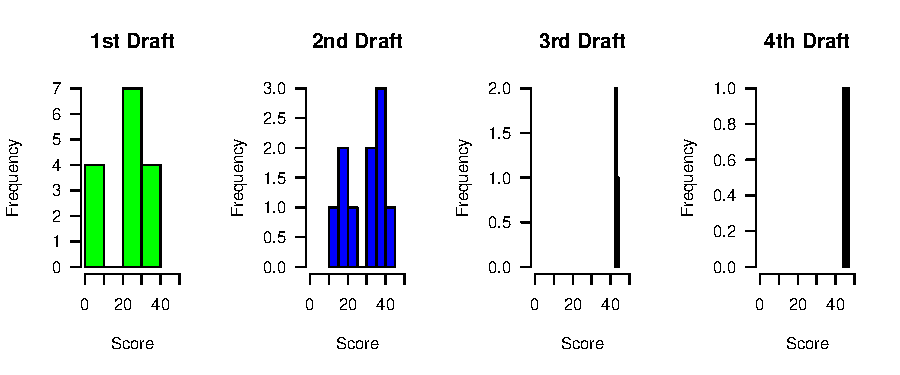
\includegraphics[width=\maxwidth]{figure/scoreshist-1} \caption[Histogram of Blog Scores]{Histogram of Blog Scores}\label{fig:scoreshist}
\end{figure}

\begin{kframe}\begin{alltt}
\hlkwd{par}\hlstd{(}\hlkwc{mfrow}\hlstd{=}\hlkwd{c}\hlstd{(}\hlnum{1}\hlstd{,}\hlnum{1}\hlstd{))}
\end{alltt}
\end{kframe}
\end{knitrout}


\section{Probability Density}

Another useful way to display data is by using probability densities (Figure~\ref{fig:scoresdensity}). Based on the normal distribution, but modified for small N, the t-distribution can be used to test the probability of differences between each draft.

\begin{knitrout}
\definecolor{shadecolor}{rgb}{0.969, 0.969, 0.969}\color{fgcolor}\begin{kframe}
\begin{alltt}
\hlstd{ttest} \hlkwb{=} \hlkwd{t.test}\hlstd{(grades1, grades2,} \hlkwc{paired}\hlstd{=F)}
\hlstd{ttestp} \hlkwb{=} \hlkwd{t.test}\hlstd{(grades1, grades2,} \hlkwc{paired}\hlstd{=T)}
\end{alltt}
\end{kframe}
\end{knitrout}

The mean was for the first draft was 21.1 and the second draft was 30.7. We can test the null hypothesis that were was no difference between the two scores. Since the difference  between the scores of the first and second submission was 9.7 points, we can reject the null hypothesis that the difference was zero using the t.test() function in R and obtain a p-value of 0.0375. We can also run the test as a pair test, where each student's first score is matched with their second score. This is useful when you have data from the same individuals; in this case the p-value is \ensuremath{10^{-4}}. However, once the probability is below 0.001, we report it as p < 0.001. 

\begin{knitrout}
\definecolor{shadecolor}{rgb}{0.969, 0.969, 0.969}\color{fgcolor}\begin{figure}
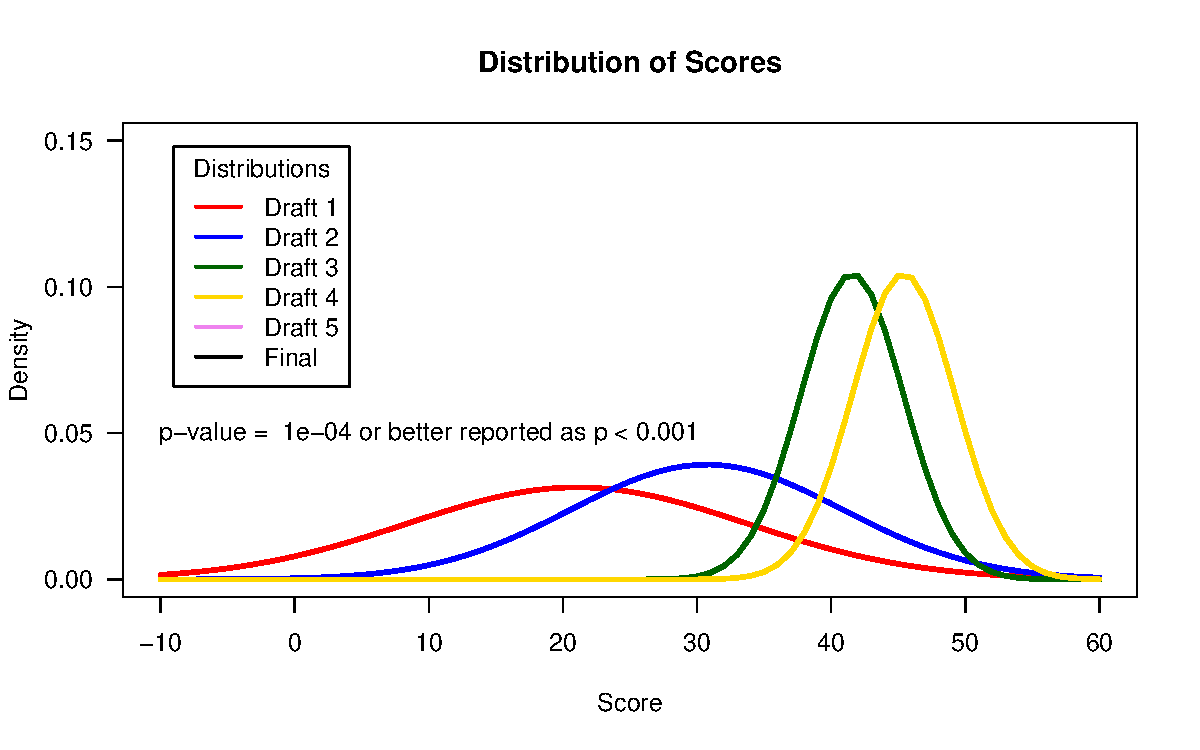
\includegraphics[width=\maxwidth]{figure/scoresdensity-1} \caption[Probability Density for Scores]{Probability Density for Scores}\label{fig:scoresdensity}
\end{figure}


\end{knitrout}

Notice how the probabilities go well beyond the scale possible, less than 0 and greater than 50. There are a number of ways of dealing with these issues, but that's beyond our scope. Suffice to say that a normal distribution is not appropriate for all data types. 

Finally, please note how the scores changed when students took full advantage of the drafting process. With each draft the mean increased, but because not everyone took advantage of the drafting process, the final mean $\bar{x}_{Final}$ was quite abit lower than that mean for scores after Draft 3, 4, and 5. 
\end{document}
